\section{\chameleon{} Prototype}

% System Design of \chameleon{}

%%%%%%%%%%%%%%%
\begin{frame}{}
  \begin{center}
    \chameleon{} prototype: \\[10pt]
    A prototype \textbf{partitioned} \textbf{replicated} \\[6pt]
    distributed transactional \textbf{key-value} store
  \end{center}
\end{frame}
%%%%%%%%%%%%%%%

%%%%%%%%%%%%%%%
\begin{frame}{}
  \begin{center}
    Classic \textbf{key-value} data model \\[4pt]
      Key: (row key, column key)
  \end{center}
\end{frame}
%%%%%%%%%%%%%%%

%%%%%%%%%%%%%%%
\begin{frame}{}
  % \fignocaption{width = 0.70\textwidth}{figs/chameleon-arch.pdf}
  \begin{center}
    \resizebox{0.70\textwidth}{!}{%        File: chameleon-arch.tex
%     Created: Mon Jan 04 08:00 PM 2016 C
% Last Change: Mon Jan 04 08:00 PM 2016 C
% 	    Used in Beamer

\begin{tikzpicture}[connection/.style = {>=Stealth, <->, brown, dashed, line width = 3pt}]
  % background: china map
  \node (china-map) [opacity = 0.20] {
\includegraphics[scale = 0.40]{figs/china-outline-blue.png}};

  % partition-left, partition-right, partition-below
  \uncover<2->{
    \node (partition-left) [] at (-6.5, 1) {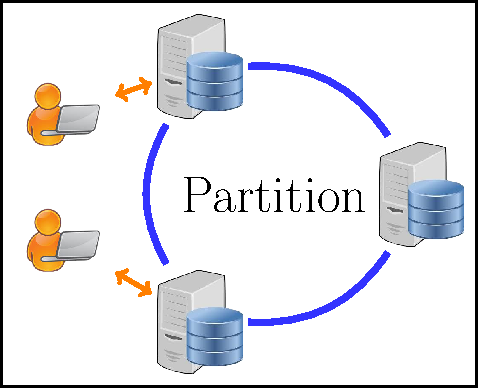
\includegraphics[scale = 0.80]{figs/partition.pdf}}; 
  }
  \uncover<3->{
    \node (partition-right) [] at (6, 3.5) {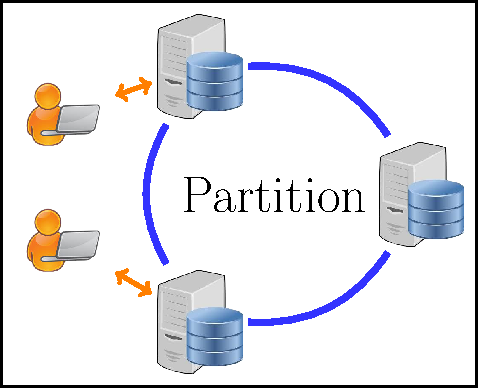
\includegraphics[scale = 0.80]{figs/partition.pdf}}; 
    \node (partition-below) [] at (1.5, -5) {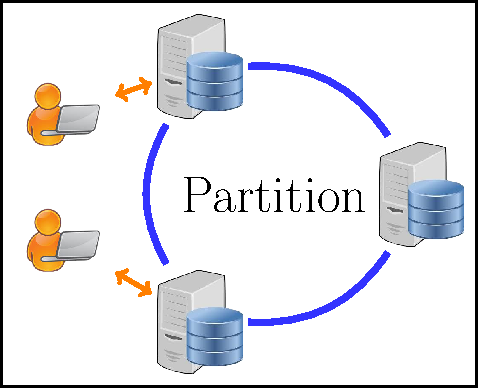
\includegraphics[scale = 0.80]{figs/partition.pdf}}; 

    % connections among partitions
    \draw [connection] (partition-left) to (partition-right); 
    \draw [connection] (partition-right) to (partition-below);
    \draw [connection] (partition-below) to (partition-left);

    % replication 
    \node (replication) [font = \Huge, align = center] at (0.5, 0.0) {\textbf{Wide-area}\\[3pt]\textbf{Replication}};
  }

  \uncover<4->{
    % master-slave for one partition
    \begin{scope}[circled/.style = {draw, circle, dash pattern = on 10pt off 5pt, cyan, line width = 2pt, outer sep = 5pt, minimum size = 2.0cm}, 
      conn/.style = {dash pattern = on 15pt off 8pt, cyan, line width = 2pt}]
    \node (ms-left) [circled] at (-4., 1) {};
    \node (ms-right) [circled] at (5.5, 1.7) {};
    \node (ms-below) [circled] at (4., -5.0) {};

    \node (master-slave) [below right = 1.5cm and -1.5cm of partition-right] {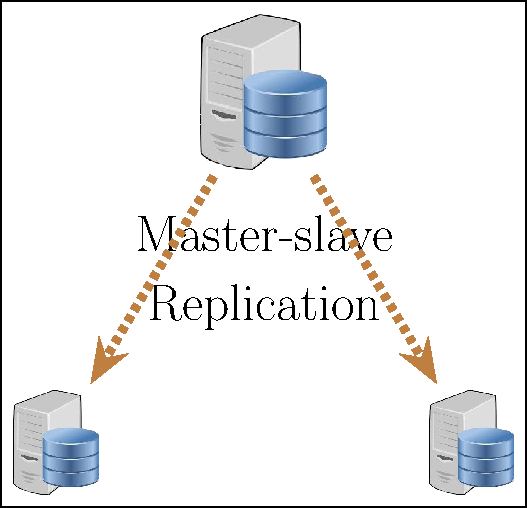
\includegraphics[scale = 0.80]{figs/master-slave.pdf}};
    \draw [conn] (ms-left) to (master-slave);
    \draw [conn] (ms-right) to (master-slave);
    \draw [conn] (ms-below) to (master-slave);
    \end{scope}
  }
\end{tikzpicture}
}
  \end{center}

  \begin{center}
    \only<2>{Keys are \textbf{partitioned} within a single datacenter.}
    \only<3-4>{Each key is \textbf{replicated} across datacenters} \only<4>{in a \textbf{master-slave} manner.}
    \only<5>{Transactions are first executed and committed on the \textbf{masters},\\
      and are then asynchronously propagated to \textbf{slaves}.}
  \end{center}
\end{frame}
%%%%%%%%%%%%%%%

%%%%%%%%%%%%%%%
\begin{frame}{}
  \only<1-3, 5->{\fignocaption{width = 0.50\textwidth}{figs/chameleon-framework.pdf}}

  \begin{center}
    \only<2>{\blue{1.} Partitioned replicated transactional key-value store}
    \only<3>{\blue{2.} Client library}
    \only<5>{\blue{3.} \rvsi{} protocol: \rvsims{} + \rvsimp{}}
  \end{center}

  \only<4>{
    Code snippet for writing \rvsi{} transactions: \\[8pt]
    \begin{lstlisting}[
  language = Java,
  basicstyle = \ttfamily\footnotesize,
  showstringspaces = false,
  keywordstyle = \color{blue}\bfseries,
  commentstyle = \color{teal},
  stringstyle = \bfseries,
  upquote = true,
  frame = box,
  breaklines = true,
  linewidth = 0.85\textwidth
]
  // Initialize keys (ck, ck1, and ck2) here
  ITx tx = new RVSITx(/** context **/);

  tx.begin();

  // Read and write
  ITsCell tsCell = tx.read(ck);
  ITsCell tsCell1 = tx.read(ck1);
  tx.write(ck1, new Cell("R1C1"));
  ITsCell tsCell2 = tx.read(ck2);

  // Specify RVSI specs. (e.g., SVSpec)
  RVSISpec sv = new SVSpec();
  sv.addSpec({ck, ck1, ck2}, 2);
  tx.collectRVSISpec(sv);

  boolean committed = tx.end();
\end{lstlisting}

  }
\end{frame}
%%%%%%%%%%%%%%%


% the RVSI-MS protocol
%%%%%%%%%%%%%%%
\begin{frame}{}
  \centerline{\rvsims{}: RVSI protocol for Master-Slave replication}

  \vspace{-0.80cm}
  \begin{center}
    \resizebox{0.50\textwidth}{!}{\begin{tikzpicture}[
  msg/.style = {>=Stealth, <->, very thick}]
  \node (ms) [] {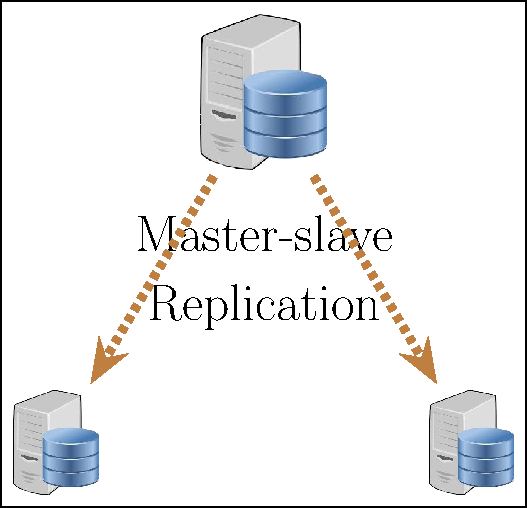
\includegraphics[scale = 0.40]{figs/master-slave.pdf}};
  \node (client) [above = 2.0cm of ms] {
\includegraphics[scale = 0.25]{figs/client-pc-logo.png}};

  \uncover<2->{
    % begin
    \draw [msg] (client) to node () [below = 5pt, midway, sloped] {\textsc{Begin}} 
    node () [above = 5pt, midway, sloped] {$T$.sts} (ms);
  }

  \uncover<3->{
    % read
    \draw [msg] (client) to [bend right = 40] node () [above = 5pt, midway, sloped] {\textsc{Read}} 
    ($(ms.south west) + (0,20pt)$);
  }

  \uncover<4->{
    % write
    \draw [msg] (client) to [out = -30, in = 30, looseness = 5] node () [] {\textsc{Write}} (client);
  }

  \uncover<5->{
    % commit
    \draw [msg] (client) to [bend left = 60] node () [below = 5pt, midway, sloped] {\textsc{Commit}} 
    node () [above = 5pt, midway, sloped] {$T$.cts} ($(ms.north) + (25pt, 0)$);
  }

  \uncover<6->{
    % vc
    \node () [below right = 0.10cm and 0.20cm of client.south, red] {$\textsc{ADD-VC}$};
    \node () [below right = 0.50cm and 0.20cm of ms.north, red] {\textsc{CHECK-VC}};
  }
\end{tikzpicture}}
  \end{center}
\end{frame}
%%%%%%%%%%%%%%%

%%%%%%%%%%%%%%%
\begin{frame}{}
  \[
    \mathcal{O}_{x}(t) = \text{version NO. of } x \text{ before time } t % \max \set{x.\attr{ord} \mid x.\attr{ts} \le t}
  \]

  % \resizebox{1.00\textwidth}{!}{\tikzset{trans-node/.style = {draw, line width = 3pt, inner sep = 12pt}}
\tikzset{read-from/.style = {>={Stealth[length = 12pt]}, ->, dash pattern = on 20pt off 10pt, thick}}
\tikzset{knode/.style = {inner sep = 8pt, outer sep = 5pt, font=\fontsize{40}{40}\selectfont}}
\tikzset{toarrow/.style = {>={Stealth[length = 12pt]}, ->, ultra thick}}
\tikzset{dashline/.style = {ultra thick, dash pattern = on 20pt off 10pt}}
\tikzset{cs/.style = {outer sep = 5pt, font=\fontsize{40}{40}\selectfont}}  % c: commit; s: start

% #1: numbering
\newcommand{\xtrans}[1]{\node (x#1) [trans-node, on chain = x, font=\fontsize{30}{30}\selectfont] {$T_{x_#1}: w_{x_#1}(x_#1)$}}
\newcommand{\ytrans}[1]{\node (y#1) [trans-node, on chain = y, font=\fontsize{30}{30}\selectfont] {$T_{y_#1}: w_{y_#1}(y_#1)$}}

\begin{tikzpicture}[start chain = x going right,
  		start chain = y going right,
	      	node distance = 1.0cm,
	        font = \huge]
  % transactions updating x
  \begin{scope}
    \foreach \i in {1, ..., 6}
      \xtrans{\i};
  \end{scope}

  % transactions updating y
  \begin{scope}
    \node (y1) [trans-node, on chain = y, below left = 3.0cm and -2.0cm of x3, font=\fontsize{30}{30}\selectfont] {$T_{y_1}: w_{y_1}(y_1)$};
    \foreach \i in {2, ..., 6}
      \ytrans{\i};
  \end{scope}
   
  % transaction T_i reading x and y
  \begin{scope}
    \node (ti) [trans-node, below right = 2.0cm and 2.5cm of y2, font=\fontsize{35}{35}\selectfont] 
	  {$T_i: \hskip 3em r_i(x_2) \hskip 8em r_i(y_5) \hskip 4em$};
  \end{scope}

  \uncover<2->{
    % T_i reads x2
    \begin{pgfonlayer}{background}
	  \coordinate (c-rx2) at ($(ti.north) !0.5! (ti.north west)$);
	  \draw[read-from]  (x2.south) to (c-rx2); % [out = -70, in = 120] (c-rx2);
    \end{pgfonlayer}
    
    % T_i reads y5
    \coordinate (c-ry5) at ($(ti.north) !0.5! (ti.north east)$);
    \draw[read-from] (y5.south) to (c-ry5);
  }

  \uncover<3->{
    % k1
    \def\konespace{11cm}
    \begin{scope}[on background layer]
	% c-x2-top: commit time of T_x2
	\draw let \p{p-x2} = (x2.east), \p{p-ti} = (ti.north west) in
	    node (c-x2-top) [cs] at ($(\x{p-x2}, \y{p-ti}) + (0.0cm, \konespace)$) {$c_{x_2}$};
	\draw[dashline] (x2.north east) to (c-x2-top.south);

	% s-ti-top: start time of T_i (drawn at the top)
	\node (s-ti-top) [cs] at ($(ti.north west) + (0.0cm, \konespace)$) {$s_i$};
	\draw[dashline] let \p{p-ti} = (ti.west), \p{p-x4} = (x4.west) in
		  (s-ti-top.south) to (\x{p-ti}, \y{p-x4});

	% k1 at center of c-x2-top and s-ti-top
	\node (k1) [knode] at ($(c-x2-top) !0.5! (s-ti-top)$) {$k_1$};
	\draw [toarrow] (k1) to (c-x2-top);
	\draw [toarrow] (k1) to (s-ti-top);
    \end{scope}
  }

  \uncover<4->{
    % k2
    \def\ktwospace{1.5cm}
    \begin{scope}[on background layer]
	% s-ti-bot: start time of T_i (drawn at the bottom)
	\node (s-ti-bot) [cs] at ($(ti.south west) - (0.0cm, \ktwospace)$) {$s_i$};
	\draw[dashline] let \p{p-ti} = (ti.west), \p{p-x4} = (x4.west) in
	(s-ti-bot.north) to (\x{p-ti}, \y{p-x4});

	% c-y5-bot: commit time of T_y5
	\draw let \p{p-y5} = (y5.east), \p{p-ti} = (ti.south west) in
	node (c-y5-bot) [cs] at ($(\x{p-y5}, \y{p-ti}) - (0.0cm, \ktwospace)$) {$c_{y_5}$};
	\draw [dashline] (y5.south east) to (c-y5-bot.north);

	% k2 at center of s-ti-bot and c-y5-bot
	\node (k2) [knode] at ($(s-ti-bot) !0.5! (c-y5-bot)$) {$k_2$};
	\draw [toarrow] (k2) to (s-ti-bot);
	\draw [toarrow] (k2) to (c-y5-bot);
    \end{scope}
  }

  \uncover<5->{
    % k3
    \begin{scope}[on background layer]
	% (invisible; as positioning anchor) s-ti-mid: start time of T_i (drawn in the middle)
	\node (s-ti-mid) [cs] at ($(s-ti-top) !0.35! (s-ti-bot)$) {};

	% c-x2-bot: commit time of T_x2 (drawn at the bottom)
	\draw let \p{p-x2} = (x2.east), \p{p-s-ti-mid} = (s-ti-mid) in
	  node (c-x2-bot) [cs] at (\x{p-x2}, \y{p-s-ti-mid}) {$c_{x_2}$};
	\draw[dashline] (x2.south east) to (c-x2-bot.north);

	% c-y5-top: commit time of T_y5 (drawn at the top)
	\draw let \p{p-y5} = (y5.east), \p{p-s-ti-mid} = (s-ti-mid) in
	  node (c-y5-top) [cs] at (\x{p-y5}, \y{p-s-ti-mid}) {$c_{y_5}$};
	\draw[dashline] (y5.north east) to (c-y5-top.south);

	% k3 at center of c-x2-bot and c-y5-top
	\node (k3) [knode] at ($(c-x2-bot) !0.5! (c-y5-top)$) {$k_3$};
	\draw [toarrow] (k3) to (c-x2-bot);
	\draw [toarrow] (k3) to (c-y5-top);
    \end{scope}
  }
\end{tikzpicture}
}

  \[
    \textcolor{teal}{r_i(x_j) \in T_i}
  \]
  \begin{center}
    \blue{The version actually observed} \emph{vs.} \red{The version just before $T_i$ starts}:
  \end{center}

  \vspace{-0.40cm}
  \begin{description}
    \item[$\konebv$:]
      \[
	\red{\mathcal{O}_{x}(T_i.\textsl{sts})} - \blue{\mathcal{O}_{x}(T_j.\textsl{cts})} < k_1
      \]
    \item[$\ktwofv$:]
      \[
	\blue{\mathcal{O}_{x}(T_j.\textsl{cts})} - \red{\mathcal{O}_{x}(T_i.\textsl{sts})} \le k_2
      \]
    \pause
      \[
	\textcolor{teal}{r_i(x_j), r_i(y_l) \in T_i} \quad (\text{Assume } T_j.\textsl{cts} < T_l.\textsl{cts})
      \]
    \item[$\kthreesv$:] The snapshot $x_j$ is born in \emph{vs.} The snapshot $y_l$ is born in:
      \[
	\mathcal{O}_{\red{x}}(T_l.\textsl{cts}) - \mathcal{O}_{\red{x}}(T_j.\textsl{cts}) \le k_3
      \]
  \end{description}
\end{frame}
%%%%%%%%%%%%%%%

% the RVSI-MP protocol
%%%%%%%%%%%%%%%
\begin{frame}{}
  \begin{center}
    \rvsimp{}: \rvsi{} protocol for Multiple Partitions\\[10pt]
    Distributed transactions spanning multiple masters \\
    need to be committed atomically.

    \pause
    \vspace{0.40cm}
    Using the two-phase commit (2PC) protocol \citeinbeamer{Bernstein}{Book}{87}.

    \pause
    \vspace{1.00cm}
    We have two issues to address.
  \end{center}
\end{frame}
%%%%%%%%%%%%%%%

%%%%%%%%%%%%%%%
\begin{frame}{}
  Assumes a global timestamp oracle \citeinbeamer{Peng}{OSDI}{10}:
  \begin{description}[Coordinator:]
    \item[Client:] asks for the start-timestamp in \textsc{Begin}
    \item[Coordinator:] asks for the commit-timestamp in \textsc{Commit}
  \end{description}
\end{frame}
%%%%%%%%%%%%%%%

%%%%%%%%%%%%%%%
\begin{frame}{}
  Split the \rvsi{} version constraints according to partitions:

  \[
    \textcolor{teal}{r_i(x_j) \in T_i}
  \]
  \vspace{-0.40cm}
  \begin{description}
    \item[$\konebv$:]
      \[
	\mathcal{O}_{\red{x}}(T_i.\textsl{sts}) - \mathcal{O}_{\red{x}}(T_j.\textsl{cts}) < k_1
      \]
    \item[$\ktwofv$:]
      \[
	\mathcal{O}_{\red{x}}(T_j.\textsl{cts}) - \mathcal{O}_{\red{x}}(T_i.\textsl{sts}) \le k_2
      \]
      \vspace{0.20cm}
      \[
	\textcolor{teal}{r_i(x_j), r_i(y_l) \in T_i}
      \]
    \item[$\kthreesv$:]
      \[
	\mathcal{O}_{\red{x}}(T_l.\textsl{cts}) - \mathcal{O}_{\red{x}}(T_j.\textsl{cts}) \le k_3
      \]
  \end{description}

  \vspace{0.6cm}
  \centerline{Each version constraint involves only one data item.}
\end{frame}
%%%%%%%%%%%%%%%
